\documentclass[spanish,12pt,a4paper,titlepage]{report}
\usepackage[utf8]{inputenc}
\usepackage{graphicx}
\usepackage{subfig}
\usepackage{float}
\usepackage{wrapfig}
\usepackage{multirow}
\usepackage{caption}
\usepackage[spanish]{babel}
\usepackage[dvips]{hyperref}
\usepackage{amssymb}
\usepackage{listings}
\usepackage{epsfig}
\usepackage{amsmath}
\usepackage{array}
\usepackage[table]{xcolor}
\usepackage{multirow}
%\usepackage[Sonny]{fncychap}
\usepackage[Lenny]{fncychap}
%\usepackage[Glenn]{fncychap}
%\usepackage[Conny]{fncychap}
%\usepackage[Rejne]{fncychap}
%\usepackage[Bjarne]{fncychap}
%\usepackage[Bjornstrup]{fncychap}

%\usepackage{subfiles}
%\usepackage{framed}

\setlength{\topmargin}{-1.5cm}
\setlength{\textheight}{25cm}
\setlength{\oddsidemargin}{0.3cm} 
\setlength{\textwidth}{15cm}
\setlength{\columnsep}{0cm}

\begin{document}

\chapter{Sniffer $i^2c$}

El cuadricóptero adquirido resuelve la comunicación entre los controladores de los motores (\textbf{ESCs}) y el microprocesador mediante el protocolo $i^2c$.\\

Para el presente proyecto resulta de vital importancia conocer dicho protocolo, ya se utilizará otro microprocesador que deberá comandar a esos mismos ESCs, supliendo el trabajo del anterior. Es entonces imprescindible conocer al detalle el funcionamiento de este protocolo, para luego poder reproducirlo.\\

Dado que no se cuenta con la colaboración de los fabricantes, y toda la información parece ser privativa, no pudiendo conseguir dato alguno de su implementación, es necesario realizar un proceso de ingeniería inversa para poder analizar, decodificar, entender y reproducir el protocolo existente. Dicho proceso de ingeniería inversa se realiza utilizando el hardware existente del cuadricóptero comercial adquirido y un analizador lógico\footnote{ChronoVu} que es capaz de leer e interpretar las líneas del bus $i^2c$ sin intervenir en las mismas.\\ \\

\begin{wrapfigure}{r}{0.5\textwidth}
	\vspace{-40pt}
	\begin{center}
	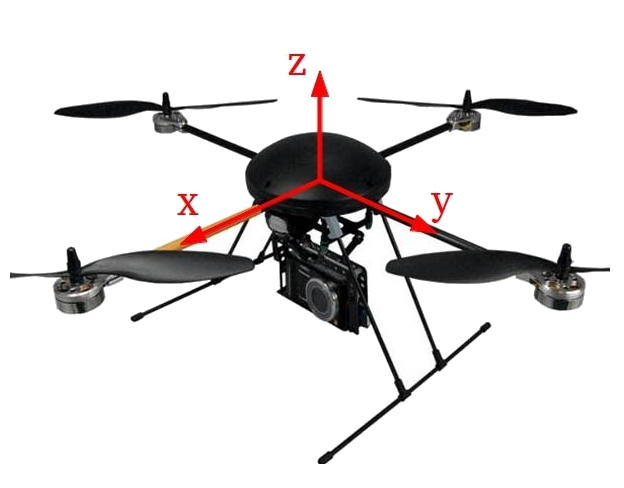
\includegraphics[width=0.4\textwidth]{./pics/ejes_quad.jpg}
	\end{center}
	\vspace{-20pt}
	\caption{Definición de ejes}
	\label{fig:ejes_quad}
	\vspace{-70pt}
\end{wrapfigure}

Antes de presentar los resultados obtenidos en el proceso, se realiza una breve introducción al protocolo $i^2c$ y se presenta en la figura \ref{fig:ejes_quad} la definición de los ejes a utilizar, lo cual será de utilidad más adelante.


\newpage
\section{Introducción al protocolo $i^2c$}

El bus $i^2c$ es un bus de comunicaciones serie. Su nombre viene de \emph{Inter-Integrated Circuit} (Circuitos Inter-Integrados).\\
Utiliza dos líneas para transmitir la información: una para los datos y otra para la señal de reloj. Además será necesaria una tercera línea de tierra, como referencia.\\
En la imagen \label{fig:setup}\footnote{Imagen tomada de www.i2c-bus.org} se muestra un diagrama de un circuito equivalente simplificado de la conexión $i^2c$ entre 2 dispositivos.

\begin{figure}[h!]
	\centering
	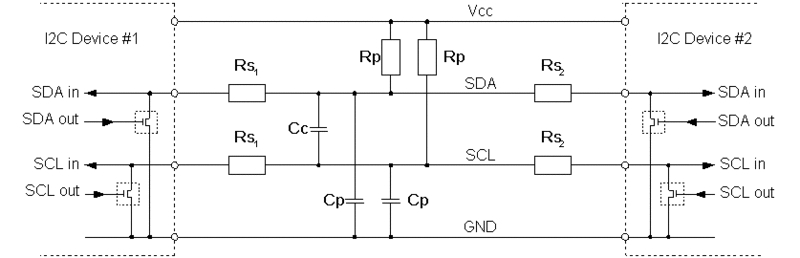
\includegraphics[width=0.8\textwidth]{./pics/setup.jpg}
	\caption{Conexión $i^2c$.}
	\label{fig:setup}
\end{figure}
donde:
\begin{verbatim}
	Vcc	 Voltaje de entrada, típicamente varía entre 1.2 V y 5.5 V
	GND	 Tierra común
	SDA	 Línea serial de datos
	SCL	 Línea serial de reloj
	Rp 	 Resistencia de "Pull-up"
	Rs 	 Resistencia serie
	Cp 	 Capacitancia del cable
	Cc 	 Capacitancia de canal cruzado
\end{verbatim}

Las líneas \textbf{SDA} y \textbf{SCL} son de drenador abierto, lo que significa que tanto el maestro como los esclavos solamente pueden conducir a nivel bajo estas líneas o dejarlos abiertos. Si ningún dispositivo $i^2c$ está conduciendo hacia abajo la línea, la resistencia de \emph{pull-up} $R_p$ se encarga de conducir la línea a $V_cc$.\\

Cada dispositivo tiene asignada una dirección que lo identifica. Para establecer una comunicación la secuencia típica empieza por el maestro enviando una secuencia de comienzo de conexión, seguida de la dirección del esclavo con el cual desea comunicarse. Seguidamente el maestro envía un bit que determina si la acción que desea realizar es escritura o lectura, a lo que el esclavo correspondiente responde con un bit de \emph{acknowledge} (\textbf{Ack}). Luego el maestro envía la dirección de memoria interna del esclavo donde debe ser almacenada la información enviada, y por último envía los datos. Para finalizar la conexión, el maestro envía una secuencia de fin de conexión.

\newpage
\section{Resultados}

Como se dijo anteriormente, para realizar el proceso de ingeniería inversa se utilizó el cuadricóptero y un analizador lógico. La forma de operar es enviar comandos conocidos con el control remoto y analizar los datos que se cursan en las líneas del bus. En la figura \ref{fig:sniffing} se muestra una foto del proceso descripto.

\begin{figure}[h!]
	\centering
	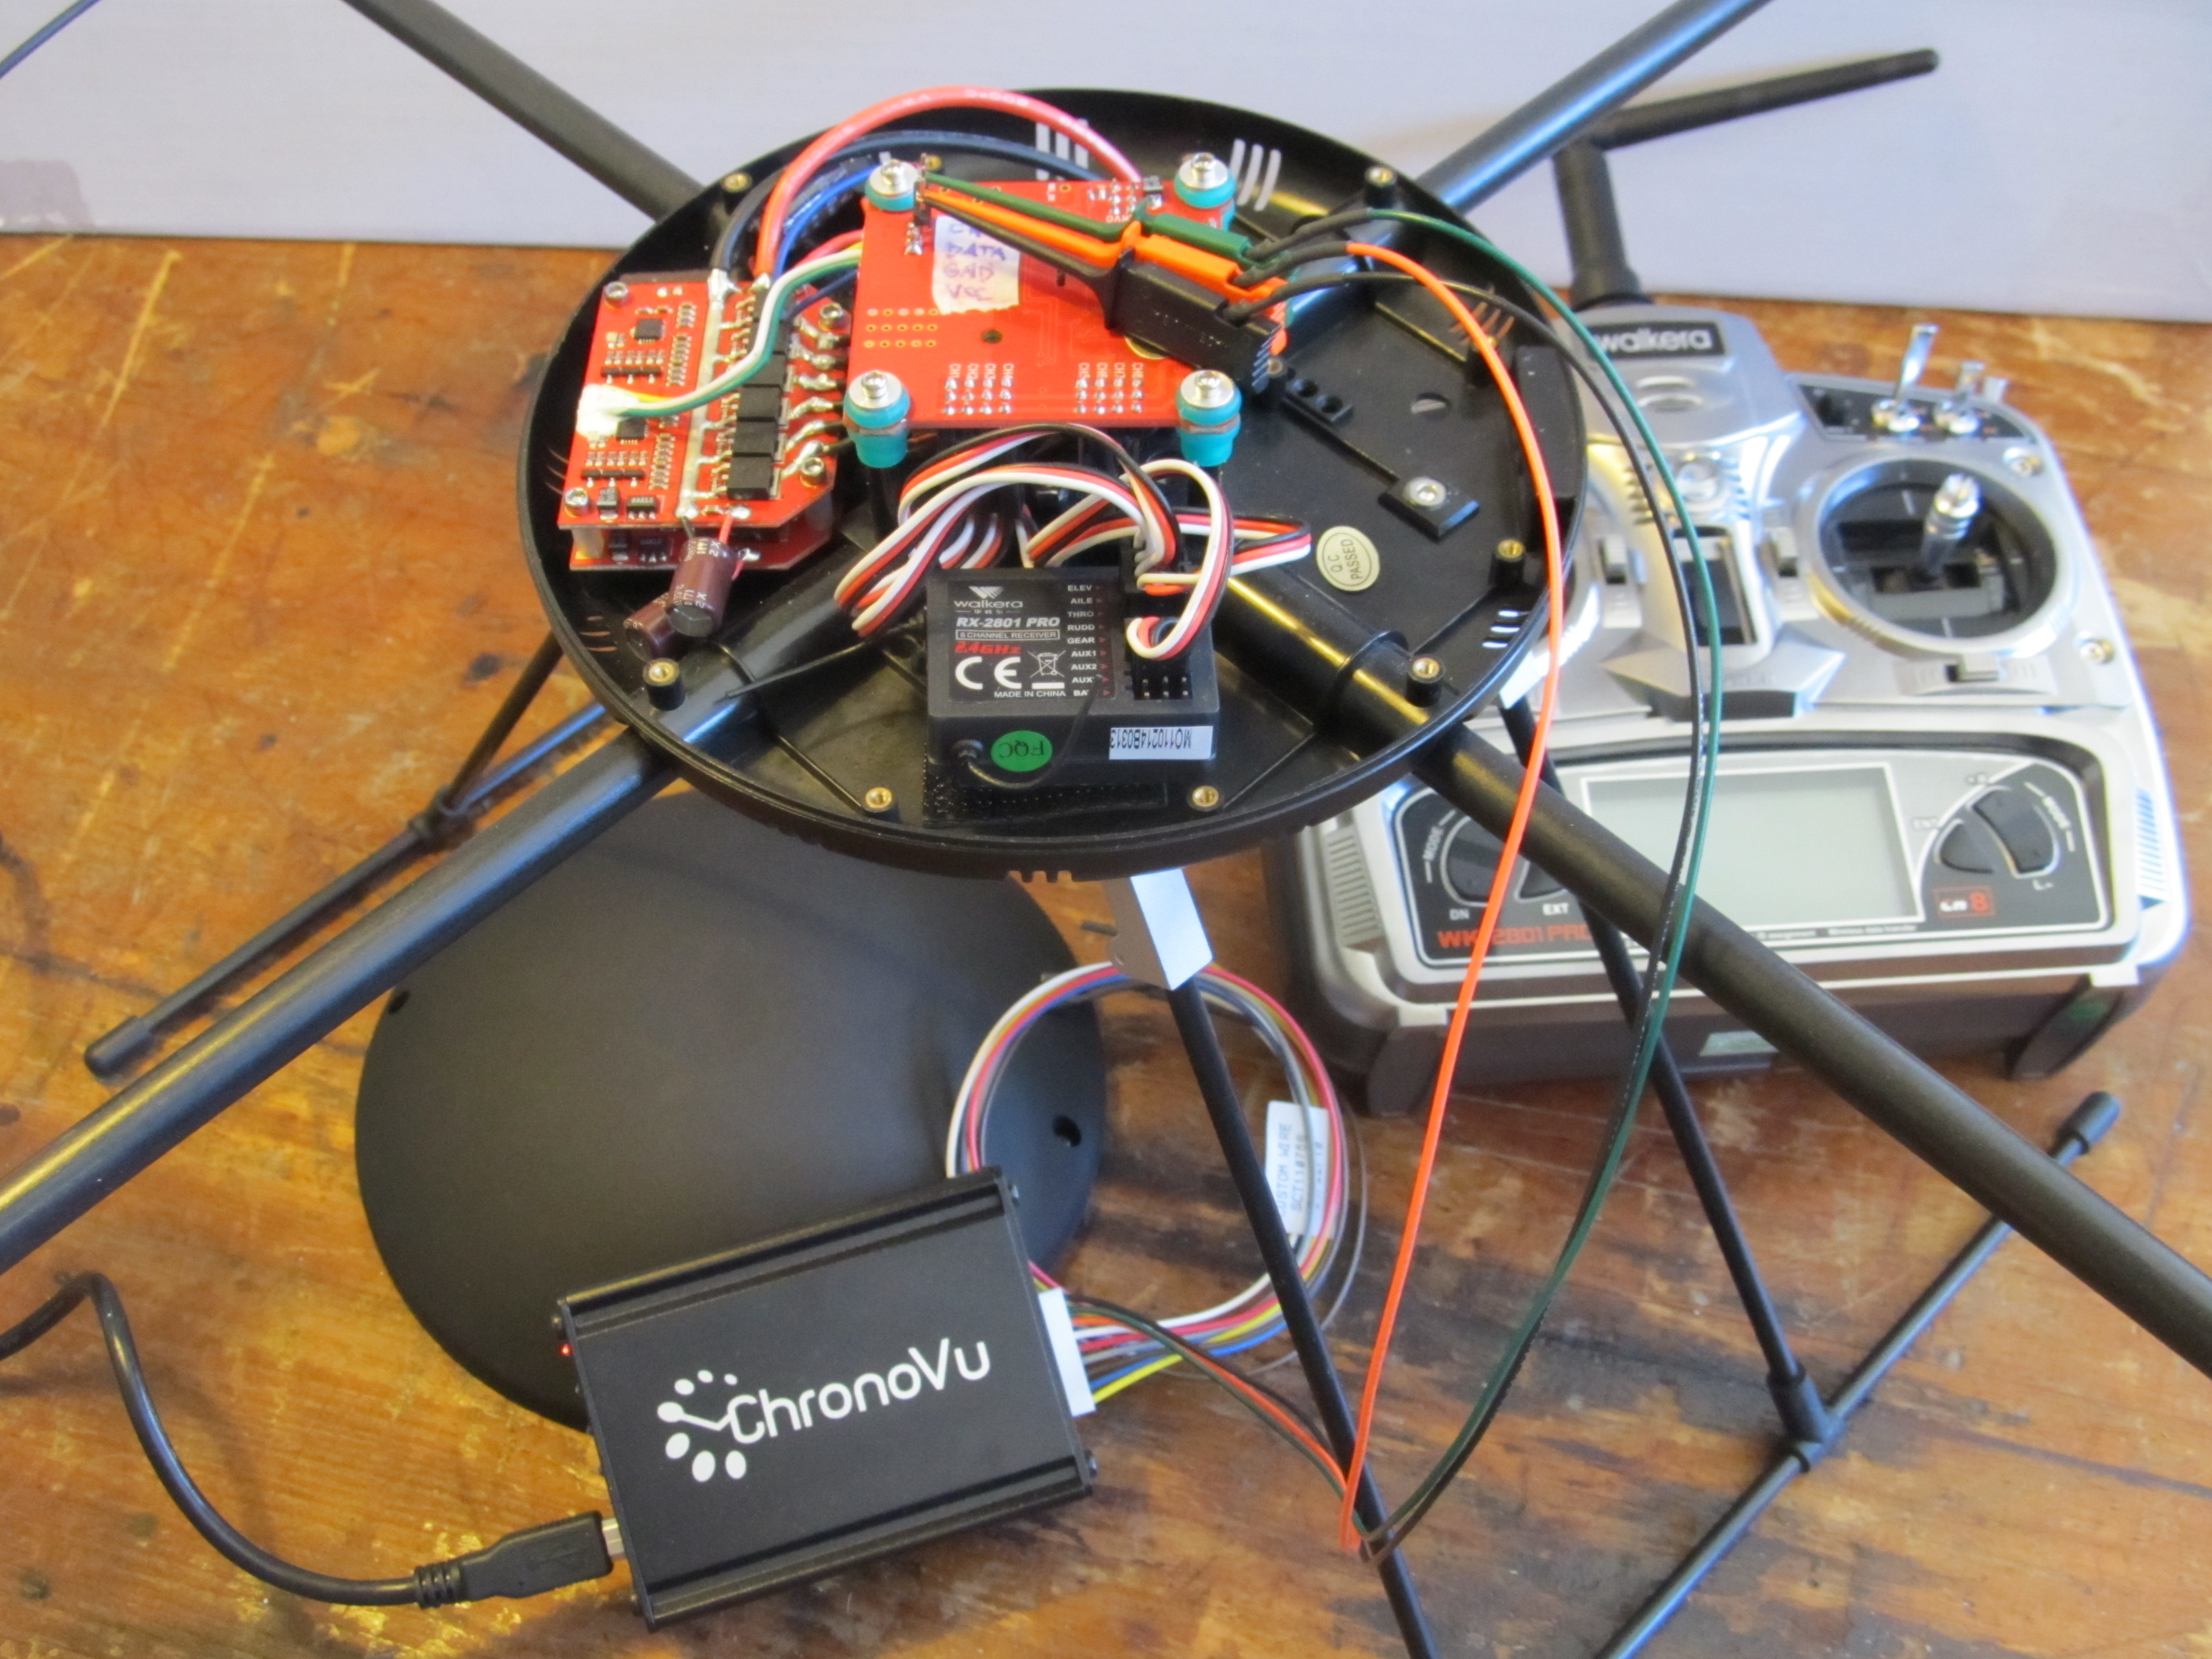
\includegraphics[width=0.6\textwidth]{./pics/sniffing.jpg}
	\caption{Proceso de lectura del bus.}
	\label{fig:sniffing}
\end{figure}

Al realizar este proceso se puede observar que se repiten cada $2ms$ bloques similares al mostrado en la figura \ref{fig:bloque_snif}.

\begin{figure}[h!]
	\centering
	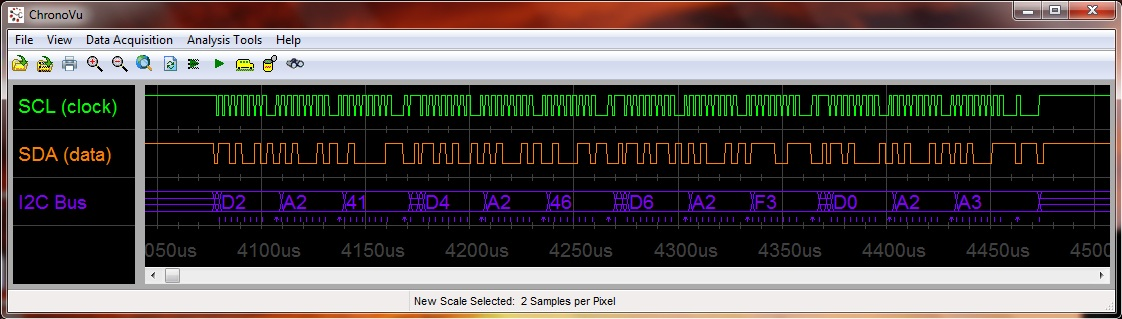
\includegraphics[width=1\textwidth]{./pics/bloque_snif.jpg}
	\caption{Bloque de transmisión $i^2c$}
	\label{fig:bloque_snif}
\end{figure}

Rápidamente, visto lo anterior, se puede deducir que hay 4 esclavos correspondientes a los 4 ESC's de los 4 motores, cuyas direcciones en hexadecimal son \textbf{D0}, \textbf{D2}, \textbf{D4} y \textbf{D6}. La dirección de la memoria interna de los esclavos donde se almacenan los datos que envía el maestro es, en todos los casos \textbf{A2}. Además el maestro envía un tercer conjunto de datos que refiere, de alguna manera, a la velocidad con la que debe girar cada motor.
Este conjunto de órdenes, agrupadas por bloques como el que se muestra en la figura \ref{fig:bloque_snif}, se repite periódicamente, indicando la velocidad con la que debe girar cada motor.\\

\subsection*{Pruebas}

Para comprender las pruebas realizadas es importante dejar en claro algunos aspectos previos. En la figura \ref{fig:tx} se muestra el transmisor utilizado para enviar comandos al cuadricóptero, un \textbf{Walkera WK-2801} y se indican los nombres de los mandos más importantes del mismo.


\begin{wrapfigure}{l}{0.55\textwidth}
	\vspace{-20pt}
	\begin{center}
	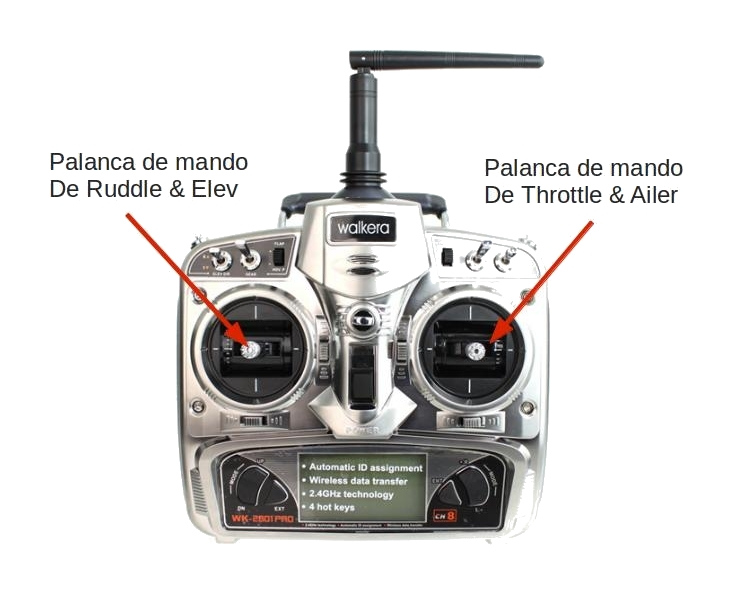
\includegraphics[width=0.45\textwidth]{./pics/tx.jpg}
	\end{center}
	\vspace{-25pt}
	\caption{Transmisor}
	\label{fig:tx}
	\vspace{20pt}
\end{wrapfigure}

Al mover el mando de la izquierda (\textbf{Elev/Rudder}) en la dirección vertical (\textbf{Elev}) se logra que el cuadricóptero se eleve verticalmente, dando igual potencia a todos los motores, mientras que al moverlo en la dirección horizontal, el cuadricóptero presenta un movimiento de rotación según su eje vertical (que pasa por el centro).\\

Al mover el mando de la derecha (\textbf{Throttle/Aile}) en la dirección horizontal (\textbf{Aile}) y vertical (\textbf{Throttle}), se logran movimientos de rotación según los ejes horizontales \emph{x} e \emph{y} del cuadricóptero. Las definiciones de los ejes se pueden ver en la figura \ref{fig:ejes_quad}.\\

Se analizan las siguientes situaciones:
\begin{table}[H]
\begin{center}
\begin{tabular}{|p{30pt}|c|c|c|c|p{130pt}|} 
\hline \cellcolor[gray]{0.8} \centering \textbf{Id} & \cellcolor[gray]{0.8} \textbf{Elev} & \cellcolor[gray]{0.8} \textbf{Ruddle} & \cellcolor[gray]{0.8} \textbf{Aile} & \cellcolor[gray]{0.8} \textbf{Throttle} & \cellcolor[gray]{0.8} \textbf{Movimiento}  \\ \hline
\centering 0 & atrás\footnote{el mínimo necesario para encender los motores} & medio & medio & medio & idle \\ \hline
\centering 1 & medio & medio & medio & medio & vertical hacia arriba con aceleración constante \\ \hline
\centering 2 & adelante & medio & medio & medio & vertical hacia arriba con aceleración constante \\ \hline
\centering 3 & medio & izquierda & medio & medio & giro según eje $z$ \\ \hline
\centering 4 & medio & derecha & medio & medio &  giro según eje $-z$ \\ \hline
\centering 5 & medio & medio & izquierda & medio & giro según eje $-x$  \\ \hline
\centering 6 & medio & medio & derecha & medio & giro según eje $x$  \\ \hline
\centering 7 & medio & medio & medio & atrás & giro según eje $-y$  \\ \hline
\centering 8 & medio & medio & medio & adelante & giro según eje $y$  \\ \hline
\end{tabular} 
\end{center}
\caption{Pruebas realizadas}
\label{tab:pruebas}
\end{table}

Se realiza un análisis de los resultados obtenidos para cada motor, graficando el contenido del byte de datos que se le transmite a cada motor. Se obtienen representaciones como la mostrada en la figura \ref{fig:grafica_motores}

\begin{figure}[h!]
	\centering
	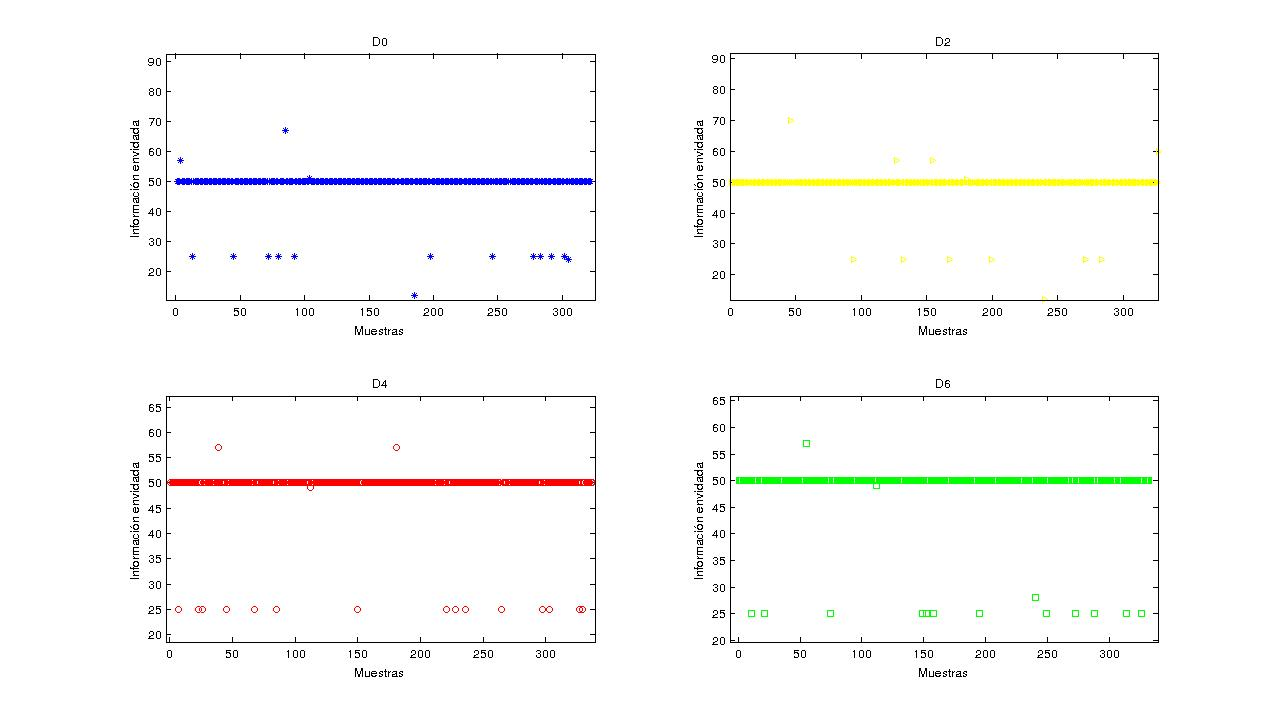
\includegraphics[width=1\textwidth]{./pics/grafica_ejemplo.jpg}
	\caption{Prueba N$^o$ $0$}
	\label{fig:grafica_motores}
\end{figure}

En la figura \ref{fig:grafica_motores} se puede observar que a los 4 motores les llega un byte con el valor promedio en $50$, el cual corresponde a la mínima potencia entregada a los motores para encenderlos.\\

Haciendo un análisis similar con el resto de las pruebas detalladas en la tabla \ref{tab:pruebas} se construye la tabla \ref{tab:resumen_snif} donde se muestran los valrores enviados a cada motor en promedio en todas las pruebas.\\

\begin{table}[H]
\begin{center}
\begin{tabular}{c|c|c|c|c|c|} 
\cline{2-5}
& \multicolumn{4}{c|}{\cellcolor[gray]{0.8} Valor promedio} \\ \hline
\multicolumn{1}{|c|}{\cellcolor[gray]{0.8} Prueba} & \cellcolor[gray]{0.8} D0 & \cellcolor[gray]{0.8} D2 & \cellcolor[gray]{0.8} D4 & \cellcolor[gray]{0.8} D6 & \cellcolor[gray]{0.8} Movimiento \\ \hline
\multicolumn{1}{|c|}{\cellcolor[gray]{0.8}0} & 50 & 50 & 50 & 50 & Idle \\ \hline
\multicolumn{1}{|c|}{\cellcolor[gray]{0.8}1} & 80 & 140 & 180 & 140 & $a_z=cte\neq 0$\\ \hline
\multicolumn{1}{|c|}{\cellcolor[gray]{0.8}2} & 180 & 220 & 250 & 240 & $a_z=cte\neq 0$ \\ \hline \hline
\multicolumn{1}{|c|}{\cellcolor[gray]{0.8}3} & 160 & 70 & 60 & 250 & giro según eje $z$ \\ \hline
\multicolumn{1}{|c|}{\cellcolor[gray]{0.8}4} & 50 & 200 & 200 & 100 & giro según eje $-z$\\ \hline \hline
\multicolumn{1}{|c|}{\cellcolor[gray]{0.8}5} & 250 & 160 & 140 & 50 & giro según eje $-x$\\ \hline
\multicolumn{1}{|c|}{\cellcolor[gray]{0.8}6} & 50 & 160 & 150 & 250 & giro según eje $x$ \\ \hline
\multicolumn{1}{|c|}{\cellcolor[gray]{0.8}7} & 90 & 50 & 250 & 160 & giro según eje $-y$\\ \hline
\multicolumn{1}{|c|}{\cellcolor[gray]{0.8}8} & 110 & 250 & 50 &  100 & giro según eje $y$\\ \hline
\end{tabular} 
\caption{Resumen de los resultados obtenidos}
\label{tab:resumen_snif}
\end{center}
\end{table}

De dicha tabla se pueden sacar algunas conclusiones importantes:
\begin{itemize}
\item La comunicación entre el amo y los esclavos por medio del protocolo $i^2c$ se lleva a cabo mediante un  formato del tipo \begin{verbatim} Dirección esclavo - Lugar de memoria donde guardar dato - dato \end{verbatim}
\item Dicho formato se repite para todos los esclavos
\item Cada esclavo recibe una actualización de estado (un dato nuevo) cada $2 ms$
\item La velocidad mínima de funcionamiento se logra enviando el valor 50
\item La velocidad máxima de funcionamiento se logra enviando el valor 250
\item La dirección de memoria interna de todos los esclavos donde se guardan los datos recibidos por el maestro es siempre 0x$A2$ (ó $162$).
\item La correspondencia entre las direcciones y los motores se muestra en la figura \ref{fig:correspondencia}. Mirando el cuadricóptero desde arriba, el motor con dirección D0 es el de la derecha, el motor con dirección D6 el de la izquierda, el D4 el de adelante y el D2 el de atrás.
% TODO
\item La suma de este m|as este es igual a la suma del otro mas el otro otro ????? Debería equilibrarse los pares no?? en las ultimas 4 pruebas deberia equilibrarse? o no?
\end{itemize}

\begin{figure}[h!]
	\centering
	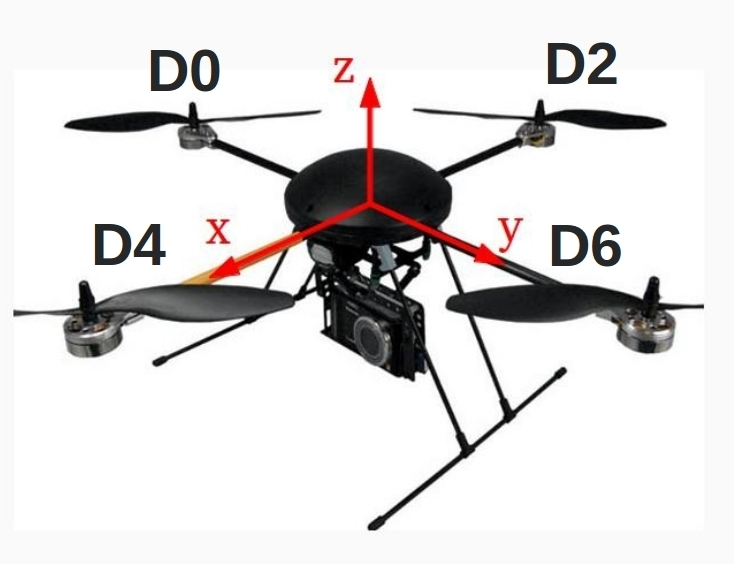
\includegraphics[width=0.4\textwidth]{./pics/correspondencias.jpg}
	\caption{correspondencias}
	\label{fig:correspondencias}
\end{figure}

\end{document}